\documentclass[10pt,a4paper]{article}

\newcommand{\COLORSDIR}{/Users/hoolywear/Desktop/UNIMORE/II ANNO/II SEMESTRE/colors}

\usepackage[italian]{babel}
\usepackage[usenames,dvipsnames]{xcolor}
\usepackage[utf8]{inputenc}
\usepackage[T1]{fontenc}
\usepackage{soul}
\usepackage[a4paper, portrait, margin=2.5cm]{geometry}
\usepackage{array}
\usepackage{tabularx}
\usepackage{multicol}
\usepackage{amsmath}
\usepackage{amsfonts}
\usepackage{amssymb}
\usepackage{algorithmicx}
\usepackage[noend]{algpseudocode}
\usepackage{wrapfig}
\usepackage{graphicx}
\graphicspath{ {./images/} }

\definecolor{emp}{HTML}{f9e9ec}
\definecolor{war}{HTML}{f88dad}
\definecolor{def}{HTML}{fac748}
\definecolor{the}{HTML}{1d2f6f}
\definecolor{obs}{HTML}{8390fa}


\usepackage{listings}

\definecolor{codeblue}{HTML}{074099}
\definecolor{codepurple}{HTML}{850075}
\definecolor{codered}{HTML}{98000f}

\lstdefinestyle{code}{
    backgroundcolor=\color{gray!10},   
    basicstyle=\ttfamily,
    breakatwhitespace=false,         
    breaklines=true,                 
    captionpos=b,                    
    keepspaces=true,                 
    showspaces=false,                
    showstringspaces=false,
    showtabs=false,                  
    tabsize=2,
    mathescape=true %dollar signs act as inline math delimiters
}
\lstdefinestyle{sql}{
    style=code,
    language=SQL,
    commentstyle=\color{codeblue},
    keywordstyle=\color{codepurple},
    stringstyle=\color{codered}
}

\lstset{style=sql}

\usepackage{mdframed}

% styles
\def\Clinewidth{.8pt}
\mdfdefinestyle{titlerule}{%
  frametitlerule=true,roundcorner=5pt,%
  frametitlerulewidth=\Clinewidth,%
  subtitleaboveline=true,subtitlebelowline=true,%
  subtitleabovelinewidth=\Clinewidth,subtitlebelowlinewidth=\Clinewidth,%
subtitlebackgroundcolor=obs,linewidth=1pt}
\mdfdefinestyle{emphasize}{%
  style=titlerule,%
  frametitle=,%
  linecolor=gray!50,linewidth=3pt,backgroundcolor=gray!10,%
  topline=false,bottomline=false,rightline=false}

% verbatim environment
\surroundwithmdframed[backgroundcolor=gray!5,hidealllines=true,%
                      innerleftmargin=1pt,innerrightmargin=1pt%
                      frametitle={}]{verbatim}

% algorithmic environment
\surroundwithmdframed[backgroundcolor=gray!10,hidealllines=true,%
frametitle={}]{algorithmic}

% quote environment
\surroundwithmdframed[style=emphasize]{quote}

% example environment
\newmdenv[frametitle=Esempio,style=titlerule]{example}

% definition environment
\newmdenv[frametitle=Definizione,style=titlerule,%
          linecolor=def]{definition}

% theorem environment
\newmdenv[frametitle=Teorema,style=titlerule,%
          linecolor=the]{theorem}

% emphasize environment
\newmdenv[style=emphasize,%
          linecolor=emp!70!red,backgroundcolor=emp]{emphasize}

% observation environment
\newmdenv[frametitle=Osservazione,%
          backgroundcolor=white,linecolor=obs,%
          frametitlebackgroundcolor=obs]{observation}

% warning environment
\newmdenv[style=emphasize,%
          backgroundcolor=war!10,linecolor=war]{warning}

\author{Iacopo Ruzzier}
\date{Ultimo aggiornamento: \today}


\title{%
Protocolli e Architetture di Rete\\
\large Appunti di teoria}

\begin{document}
\maketitle
\tableofcontents
\newpage
\section{Introduzione a reti e protocolli}

\subsection{Reti}

\begin{minipage}[c]{.6\textwidth}
Essendo difficile dare una definizione globale di rete, vediamone una \textbf{ricorsiva}: rete come
\begin{itemize}
  \item insieme di \textbf{nodi} connessi tramite \textbf{collegamenti}
  \item insieme di \textbf{reti} connesse tramite \textbf{nodi}
\end{itemize}
La definizione introduce una prima astrazione: quando inseriamo una rete all'interno di una rete pi\`u grande, \textbf{non ci interessa come \`e fatta la singola rete} al suo interno
\end{minipage}
\begin{minipage}[c]{.4\textwidth}
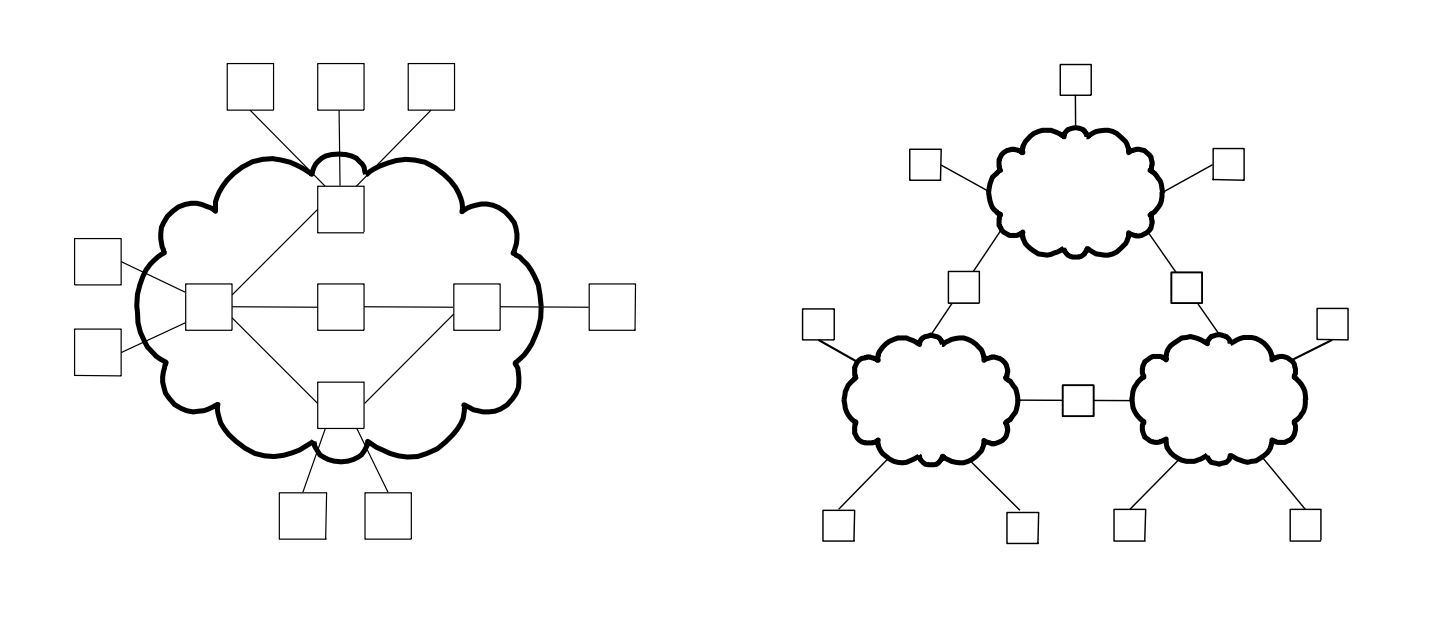
\includegraphics[width=\textwidth]{teoria_intro_1.png}
\captionof{figure}{Definizione ricorsiva di rete}
\end{minipage}

\subsubsection{Componenti fondamentali}

\begin{itemize}
  \item \textbf{nodi} $\rightarrow$ distinti per \textbf{ruolo}
    \begin{itemize}
      \item host: termine astratto, identifica un \textbf{nodo terminale} (mittente o destinatario, dunque connesso ad un capo della comunicazione)
      \item switch, bridge, router: nodi intermedi che abilitano la comunicazione tra host
      \begin{emphasize}
          Vedremo che gli host devono implementare \textbf{tutti i protocolli di rete}, mentre i nodi intermedi possono conoscerne anche solo una parte (costo decisamente minore)
      \end{emphasize}
      
    \end{itemize}
  \item \textbf{collegamenti (link)}: tutti i mezzi fisici usati per comunicare, cablati e non (wireless)
\end{itemize}

La definizione ricorsiva permette l'uso di \textbf{paradigmi di astrazione}: nascondo dettagli per focalizzarmi su funzionalit\`a di interesse\\
Inoltre, l'approccio ricorsivo permette il \textbf{riutilizzo}

\begin{example}[frametitle={Esempio: passaggio di informazioni tra host in LAN diverse}]
 \noindent\textit{
    LAN/WAN: Local/Wide Area Network; gli host si connettono alle LAN, le WAN collegano le LAN
  }

  \noindent\begin{minipage}[c]{.6\textwidth}
  \textit{Logicamente} comunicano i due host terminali, ma in realt\`a le informazioni \textbf{attraversano tutti i nodi e collegamenti intermedi} $\rightarrow$ sorgono problemi di
  \begin{itemize}
    \item \textbf{instradamento} - che direzione far prendere al messaggio
    \item \textbf{condivisione delle risorse} - un nodo condiviso da vari host avr\`a prestazioni \textbf{variabili}
  \end{itemize}
  \begin{emphasize}
    L'obiettivo, apparentemente semplice, di trasferire un messaggio in forma di sequenza di bit da un host a un altro, \`e in realt\`a difficile da raggiungere al meglio
  \end{emphasize}
  \end{minipage}\hfill
  \begin{minipage}[c]{.3\textwidth}
  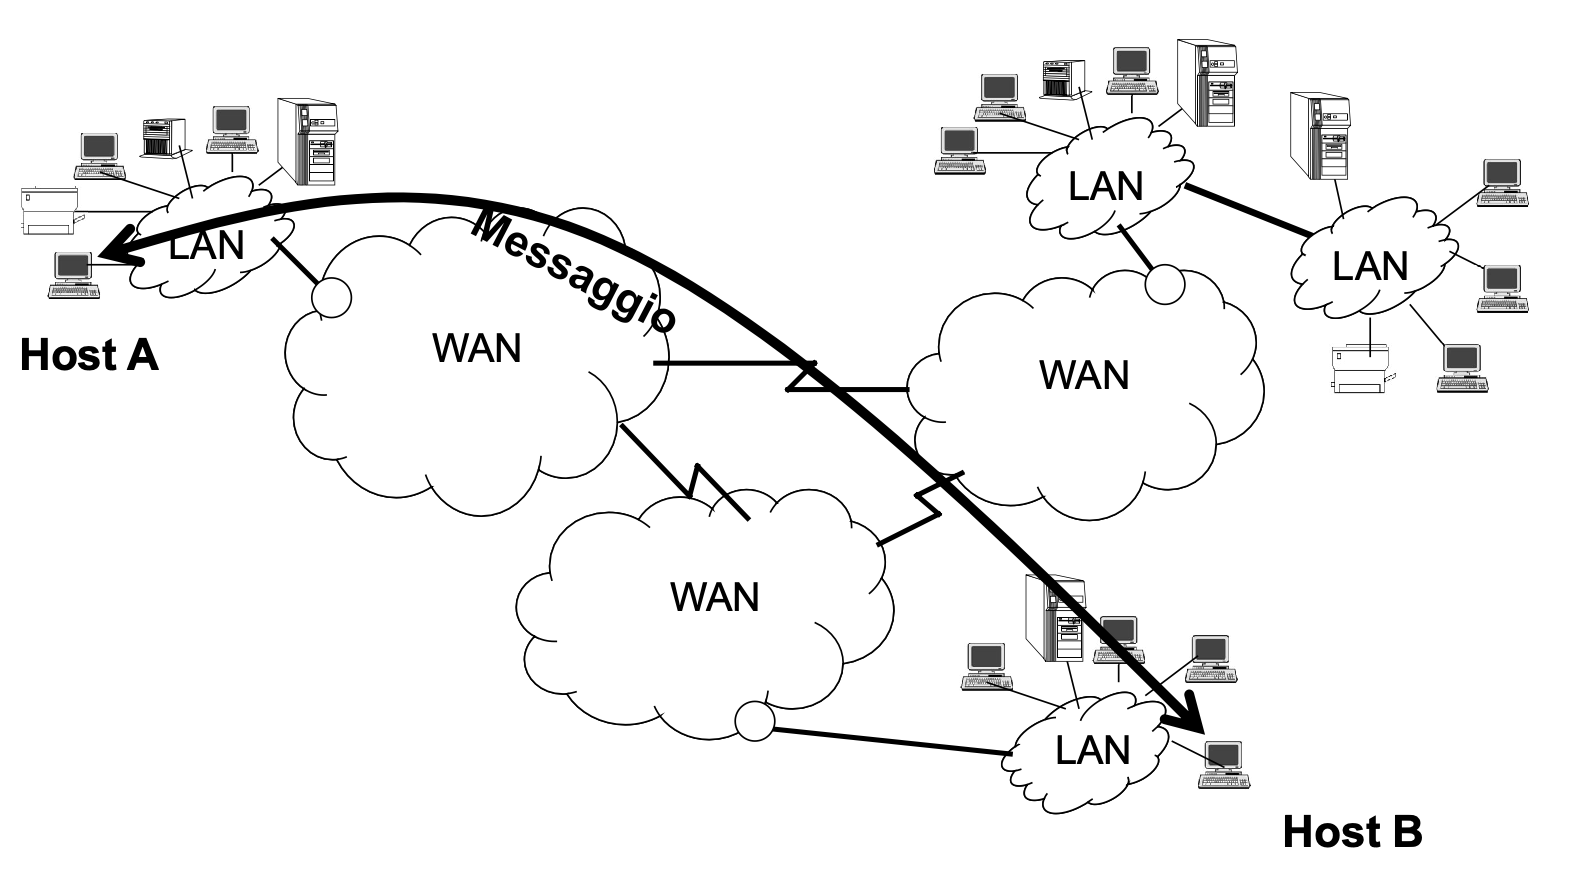
\includegraphics[width=\textwidth]{teoria_intro_2.png}
  \captionof{figure}{comunicaz.~logica}
  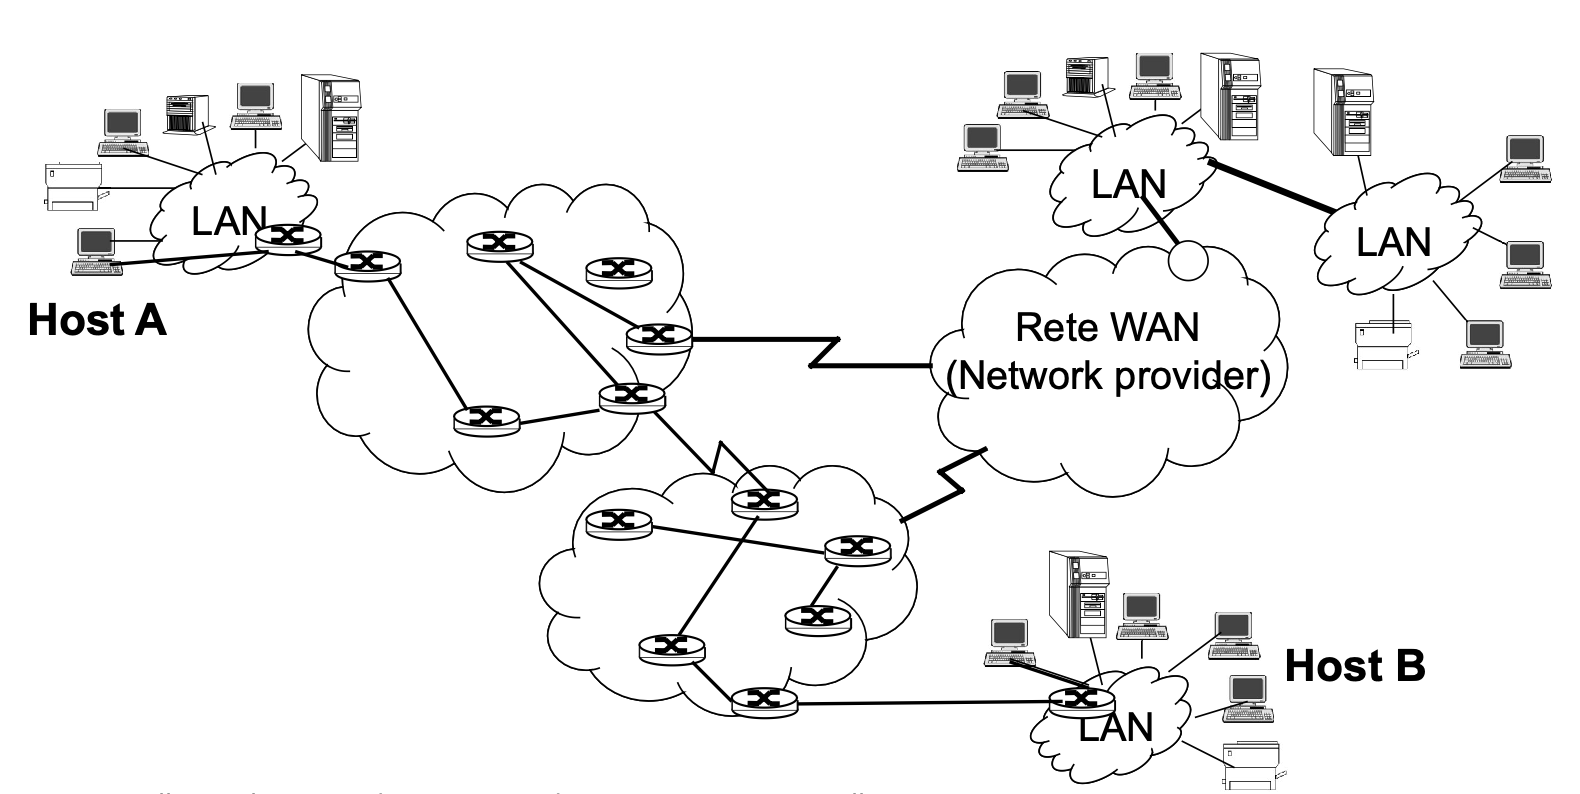
\includegraphics[width=\textwidth]{teoria_intro_3.png}
  \captionof{figure}{comunicaz.~reale}
  \end{minipage}
  
\end{example}

\vspace{-10pt}
\subsubsection{Aspetti fondamentali delle reti moderne}

\begin{itemize}
  \item host, nodi, link \textbf{eterogenei} $\rightarrow$ \textbf{sia HW che SW}
  \item la rete pu\`o \textbf{cambiare nel tempo} (es.~aggiunta di host a comunicazione iniziata)
  \item \textbf{compromessi} per ottenere i massimi benefici:
  \begin{itemize}
    \item \textbf{costi} vs \textbf{prestazioni} vs \textbf{affidabilit\`a} vs \textbf{sicurezza}
    \item condivisione della rete
  \end{itemize}
\end{itemize}
\newpage % MIGHT CAUSE ERRORS IN THE FUTURE ("absolute" positioning)
L'estrema eterogeneit\`a ci porta a preoccuparci di
\begin{multicols}{2}
\begin{itemize}
  \item diversit\`a HW/SW dei nodi
  \item com'\`e interconnesso l'host
  \item modalit\`a di trasmissione del messaggio
  \item gestione del transito attraverso i n. intermedi
  \item servizi disponibili all'utente
  \item ...
\end{itemize}
\end{multicols}

\textbf{Difficolt\`a} (tutto pu\`o andare storto):
\begin{multicols}{2}
\begin{itemize}
  \item interferenze elettriche (errori a livello di bit)
  \item congestioni (errori a livello di messaggi)
  \item guasti link/n.~intermedi
  \item problemi SW di host
\end{itemize}
\end{multicols}


$\rightarrow$ \textbf{ritardi, consegne fuori ordine, "ascolto da terzi"...}

$\Rightarrow$ per far comunicare tra loro delle entit\`a di una rete, tenendo conto di tutte le problematiche e circostanze, si richiede \textbf{cooperazione}: \textbf{tutte le comunicazioni sono regolate da \underline{protocolli}}

\subsection{Protocolli}

\textbf{Protocollo}: insieme di \textbf{regole e convenzioni} seguite da entit\`a, dislocate \textbf{su nodi distinti}, che intendono \textbf{comunicare per svolgere un compito comune}

Obiettivo: assicurare una cooperazione \textbf{efficiente e affidabile} per la comunicazione e per la realizzazione di servizi di rete

\begin{emphasize}
    Il singolo protocollo \textbf{non pu\`o risolvere tutti i problemi}! Usiamo pr. diversi a seconda del contesto e del nostro scopo
\end{emphasize}

\subsubsection{Elementi fondamentali (e rigorosi)}

\begin{minipage}[c]{.6\textwidth}
\begin{itemize}
  \item \textbf{sintassi}: insieme delle \textbf{informazioni ammissibili} $\rightarrow$ insieme e struttura di comandi e risposte, formato dei messaggi, ... (correttezza a livello di "parola" - "presenza della parola nel dizionario")
  \item \textbf{semantica}: \textbf{significato} di comandi, azioni, risposte in seguito a ricezione e trasmissione dei messaggi ("sequenze ammissibili di aprole per formare frasi di senso computo")
  \item \textbf{temporizzazione}: specifica delle possibili \textbf{sequenze temporali di emissione di comandi, messaggi, risposte} ("seq.~ammissibili di frasi per un discorso di senso compiuto")
\end{itemize}
\end{minipage}
\begin{minipage}[c]{.4\textwidth}
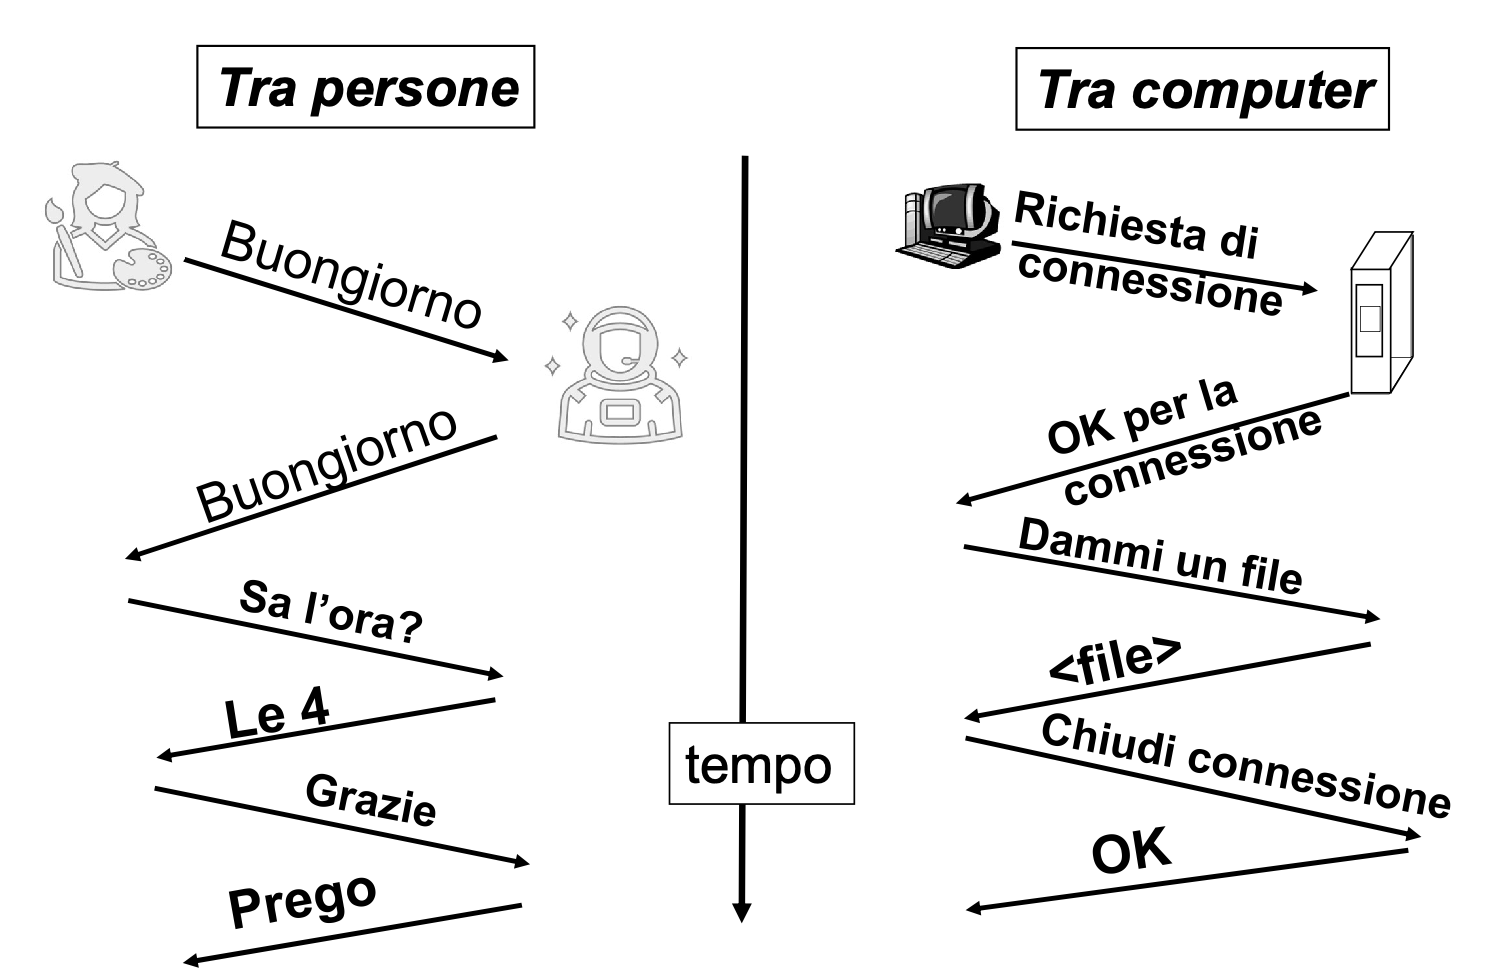
\includegraphics[width=\textwidth]{teoria_intro_4.png}
\captionof{figure}{Esempi di comunicazione}
\end{minipage}


\begin{emphasize}
  A differenza del linguaggio comune, dove qualche parola sbagliata non interferisce con la comprensione del messaggio, nelle reti informatiche pu\`o essere sufficiente un errore di pochi bit
\end{emphasize}

\begin{example}[frametitle={4 domande fontamentali per la comunicazione tra entit\`a}]
  \begin{enumerate}
    \item \textbf{architettura HW}~\begin{minipage}[t]{.5\textwidth}
        \begin{itemize}
          \item[$\rightarrow$] quale HW esegue il protocollo
          \item[$\rightarrow$] dove viaggia l'informazione
        \end{itemize}
      \end{minipage}
    \item \textbf{schema di naming/identificazione} $\rightarrow$ come si chiamano gli interlocutori
    \item \textbf{architettura SW} $\rightarrow$ quale SW esegue il protocollo
    \item \textbf{schema di comunicazione} $\rightarrow$ quale paradigma di comunicazione voglio usare
  \end{enumerate}
\end{example}

\subsubsection{Stack di protocolli}

Il vero obiettivo \`e il \textbf{trasferimento di un messaggio, garantendo}
\begin{itemize}
  \item \textbf{prestazioni} (massima velocit\`a possibile)
  \item \textbf{affidabilit\`a} (superamento di guasti o malfunzionamenti)
  \item \textbf{sicurezza}
\end{itemize}

In un contesto eterogeneo rendono il problema non banale: si usa un approccio \textit{divide et impera}, che in ambito informatico si concretizza usando astrazioni per mascherare la complessit\`a\\
$\rightarrow$ approccio stratificato (layering), realizzando uno \textbf{stack (o suite) di protocolli} in cui ogni livello cerca di risolvere un problema diverso

\begin{emphasize}
    Quasi mai i nodi sono i singoli PC, bens\`i le varie \textbf{applicazioni in esecuzione (processi)}
\end{emphasize}

\noindent\begin{minipage}[c]{.5\textwidth}
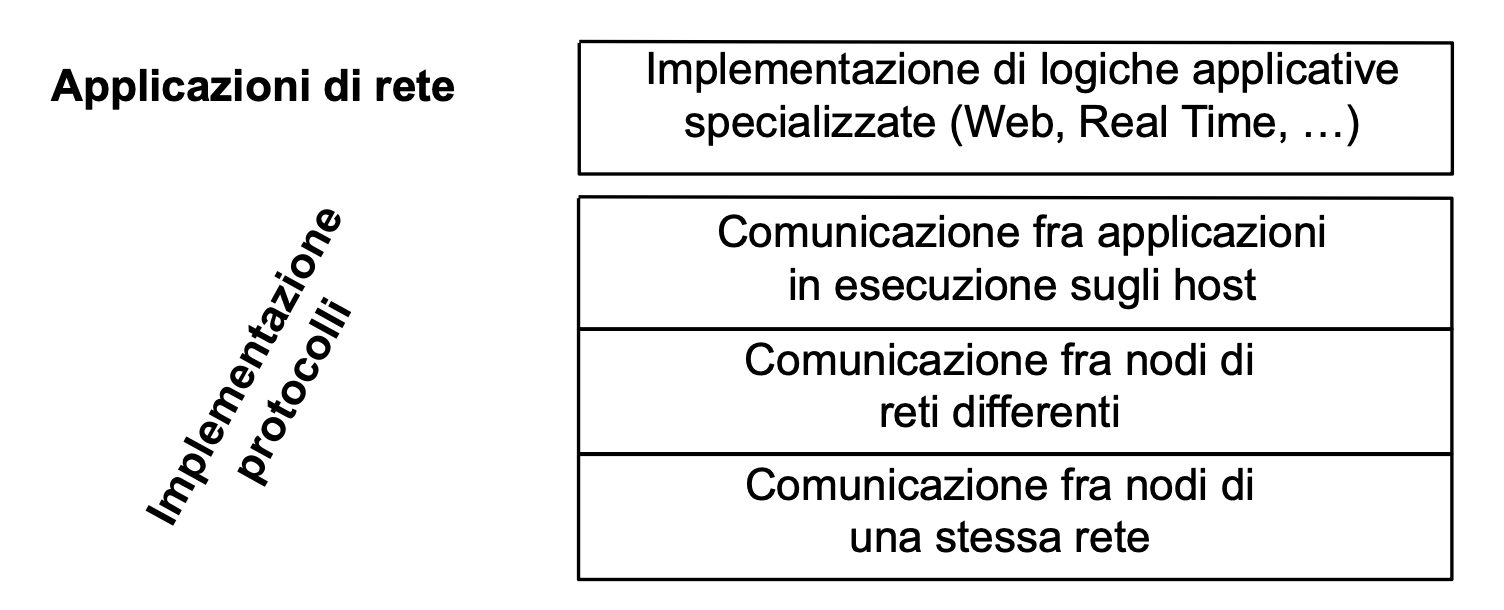
\includegraphics[width=\textwidth]{teoria_intro_5.png}
\captionof{figure}{Esempio concettuale semplificato}
\end{minipage}
\begin{minipage}[c]{.5\textwidth}
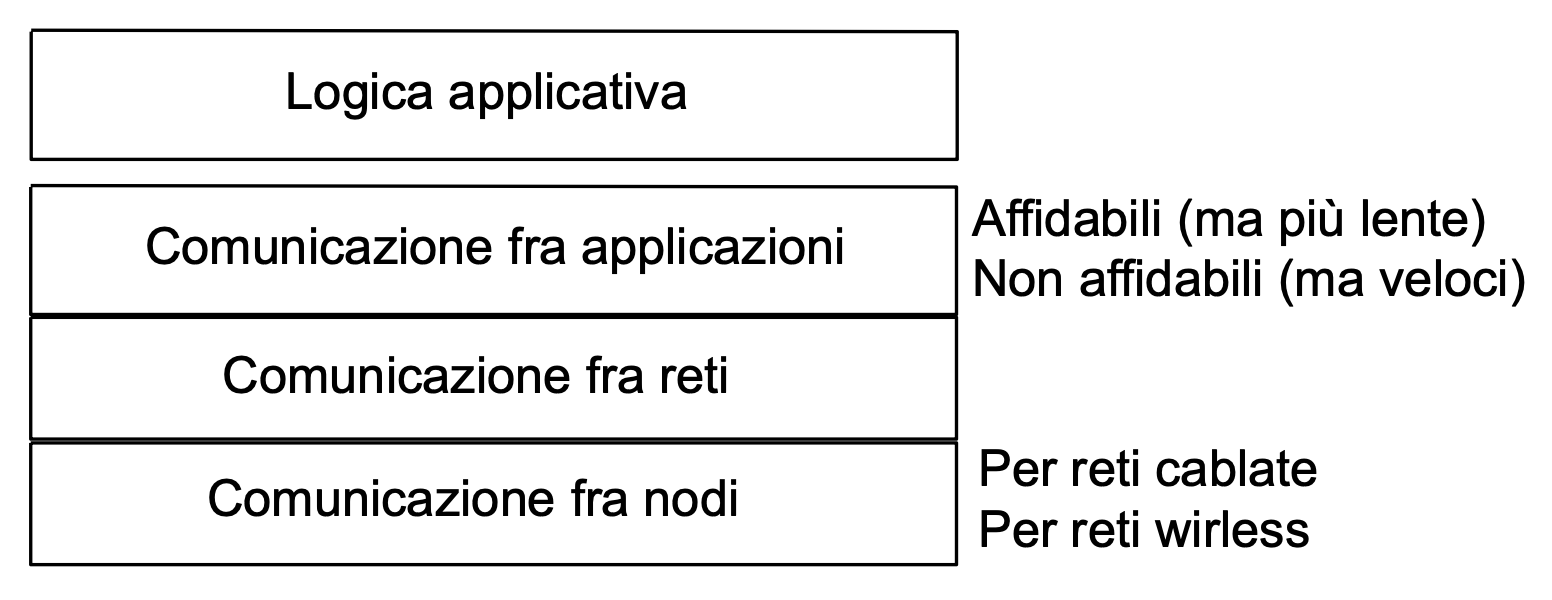
\includegraphics[width=\textwidth]{teoria_intro_6.png}
\captionof{figure}{Termini pi\`u generici}
\end{minipage}\\

Il livello 1 \`e quello \textbf{HW} (ci interessa meno), e pi\`u saliamo pi\`u ci avviciniamo alla logica applicativa. I livelli superiori possono essere variabili, e ciascun livello pu\`o offrire protocolli "alternativi" a seconda dell'aspetto da sostenere (es.~affidabilit\`a vs velocit\`a - una telefonata \`e preferibile in tempo reale, anche se perdo qualche parola ogni tanto)\\
In termini logici, salendo di livello le comunicazioni avvengono \textbf{sulla stessa rete locale} (1\textsuperscript{o}) $\rightarrow$ \textbf{su reti diverse} (2\textsuperscript{o}) $\rightarrow$ \textbf{tra nodi} (3\textsuperscript{o})

\begin{emphasize}
    Lo stack pu\`o "aumentare verso l'alto" indefinitamente, mentre i primi 3 livelli ci sono sempre
\end{emphasize}

\noindent\begin{minipage}[c]{.7\textwidth}
Ogni livello ha
\begin{itemize}
  \item 2 interfacce \textbf{interne}, rivolte verso i livelli superiore e inferiore
  \item 1 interfaccia \textbf{esterna}, per comunicazioni tra mittente e destinatario \textit{sullo stesso livello}
\end{itemize}
\end{minipage}
\begin{minipage}[c]{.3\textwidth}
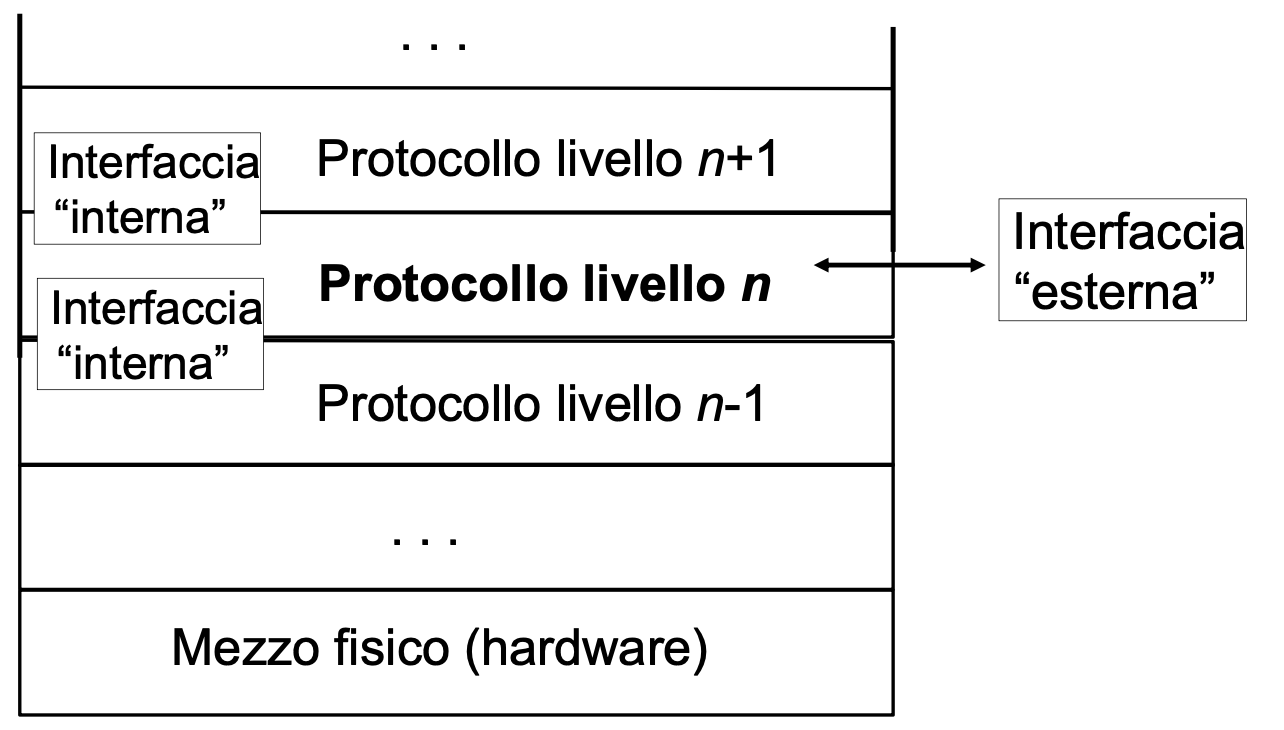
\includegraphics[width=\textwidth]{teoria_intro_7.png}
\captionof{figure}{Interfacce a livello $n$}
\end{minipage}\\

\textbf{Concettualmente e logicamente}, la comunicazione avviene tra \textbf{protocolli allo stesso livello}. In realt\`a avviene in modo diretto solo al livello \textbf{pi\`u basso} (attraverso il mezzo fisico), mentre per gli altri \`e indiretta: il messaggio \textit{scende} dal livello applicativo a quello fisico (mittente), per poi \textit{risalire} lo stack (destinatario).

\noindent\begin{minipage}[c]{.5\textwidth}
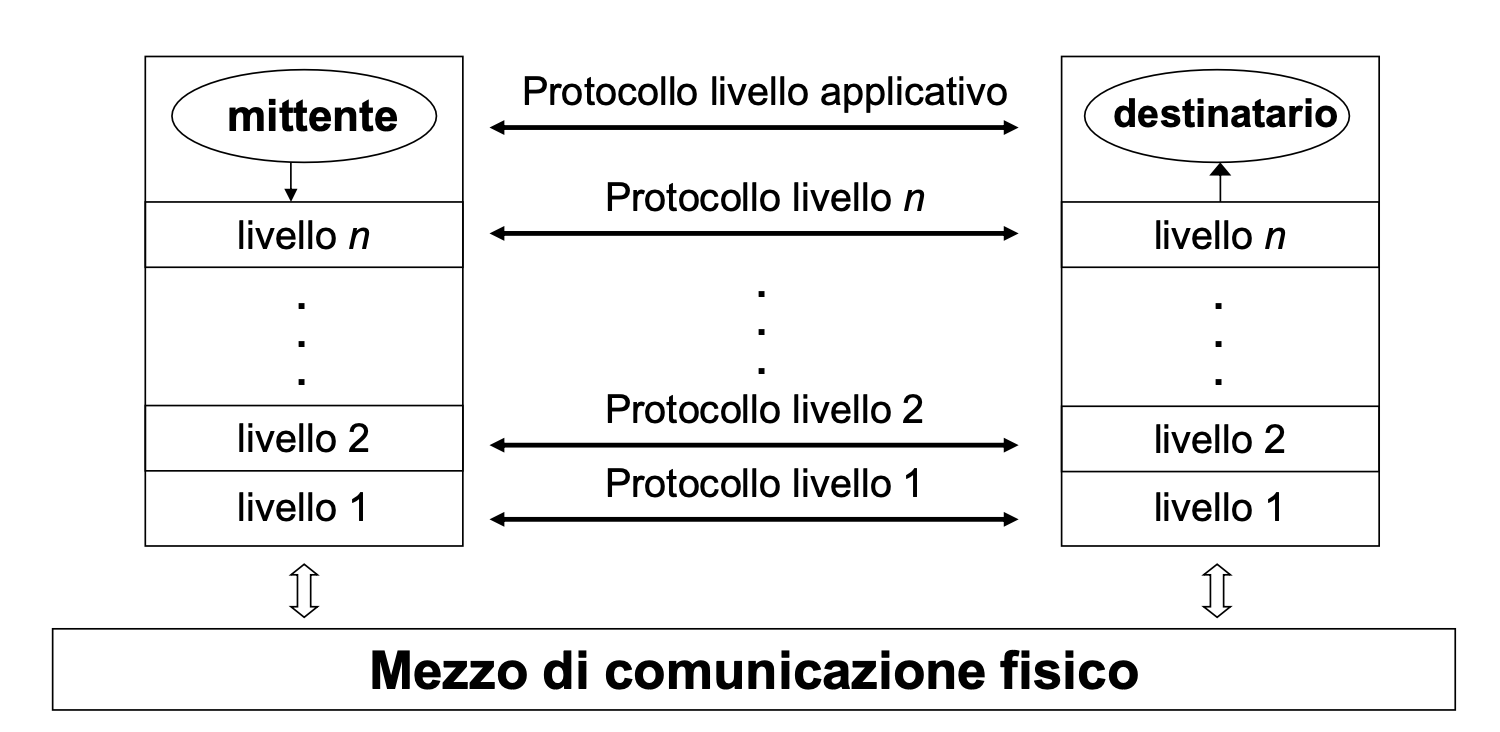
\includegraphics[width=\textwidth]{teoria_intro_8.png}
\captionof{figure}{Comunicazione logica}
\end{minipage}
\begin{minipage}[c]{.5\textwidth}
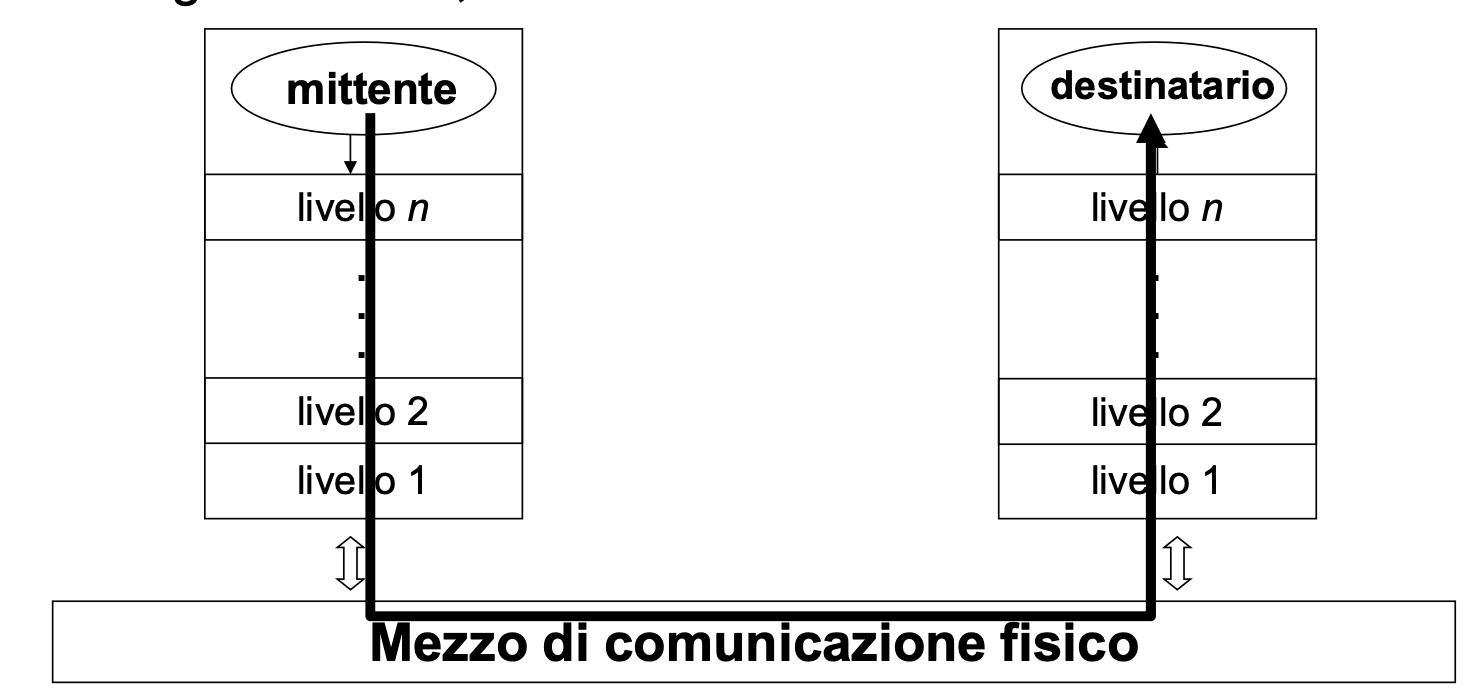
\includegraphics[width=\textwidth]{teoria_intro_9.png}
\captionof{figure}{Comunicazione fisica}
\end{minipage}\\

Possiamo dire che ogni protocollo del mittente parla con lo stesso protocolo del destinatario. 

\subsubsection{Pacchetti}

\noindent\begin{minipage}[c]{.7\textwidth}
In termini di protocollo, l'unit\`a minima di comunicazione \`e il \textbf{pacchetto}, struttura dati composta da
\begin{itemize}
  \item \textbf{PCI} (Protocol Control Information) o \textbf{header}: insieme di tutti i metadati necessari per il funzionamento del protocollo
  \item \textbf{SDU} (Service Data Unit) o \textbf{payload}: il verto contenuto informativo scambiato
\end{itemize}
In generale, PCI+SDU=\textbf{PDU} (Protocol Data Unit)
\end{minipage}\hfill
\begin{minipage}[c]{.25\textwidth}
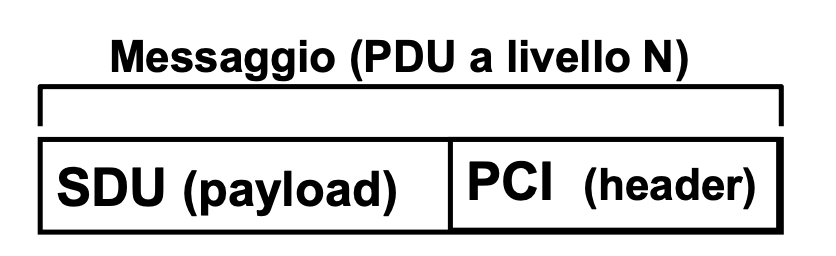
\includegraphics[width=\textwidth]{teoria_intro_10.png}
\captionof{figure}{Struttura del pacchetto a livello $n$}
\end{minipage}

\paragraph{Implementazione dell'interfaccia esterna}~\\

\noindent\begin{minipage}[c]{.7\textwidth}
\begin{itemize}
  \item quando un livello invia un messaggio, invia \textbf{l'intero PDU} a sua disposizione al livello pi\`u basso
  \item il livello inferiore \textbf{aggiunge il proprio header} al PDU ricevuto (rimane inalterato)
  \item a liv.~1 avremo molto payload + header liv.~1
  \item quando il messaggio arriva al destinatario, ogni livello \textbf{toglie l'header} del suo protocollo e \textbf{inoltra il suo payload} al liv.~superiore
\end{itemize}
\captionof{figure}{Schema di funzionamento dell'incapsulamento e della gerarchia}
\end{minipage}\hfill
\begin{minipage}[c]{.25\textwidth}
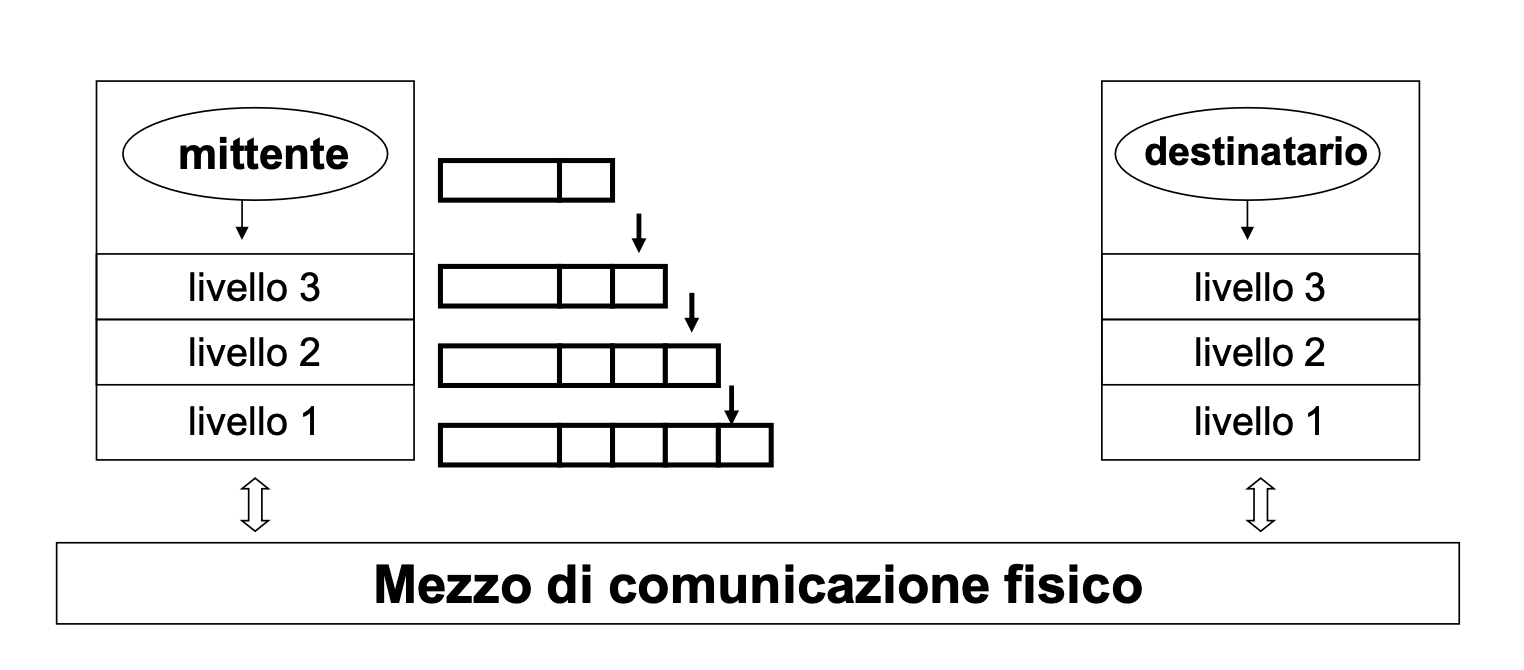
\includegraphics[width=\textwidth]{teoria_intro_11.png}
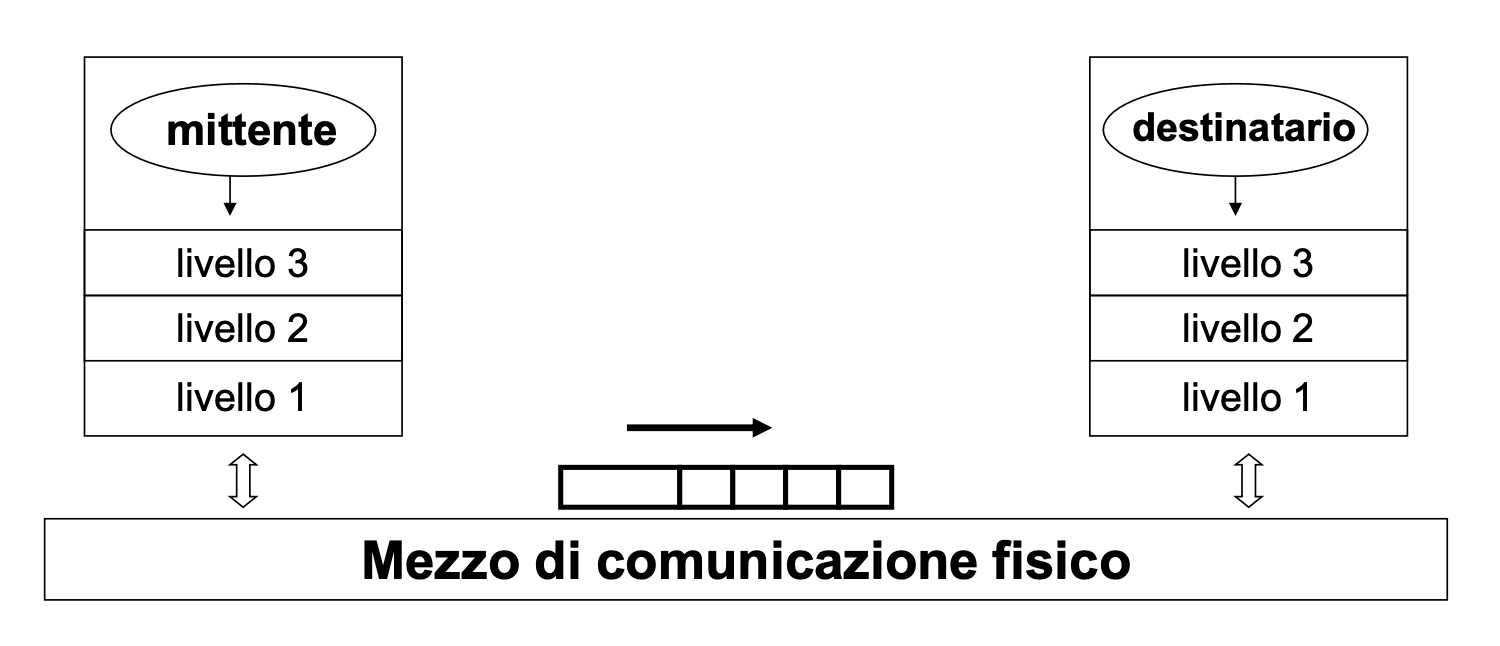
\includegraphics[width=\textwidth]{teoria_intro_12.png}
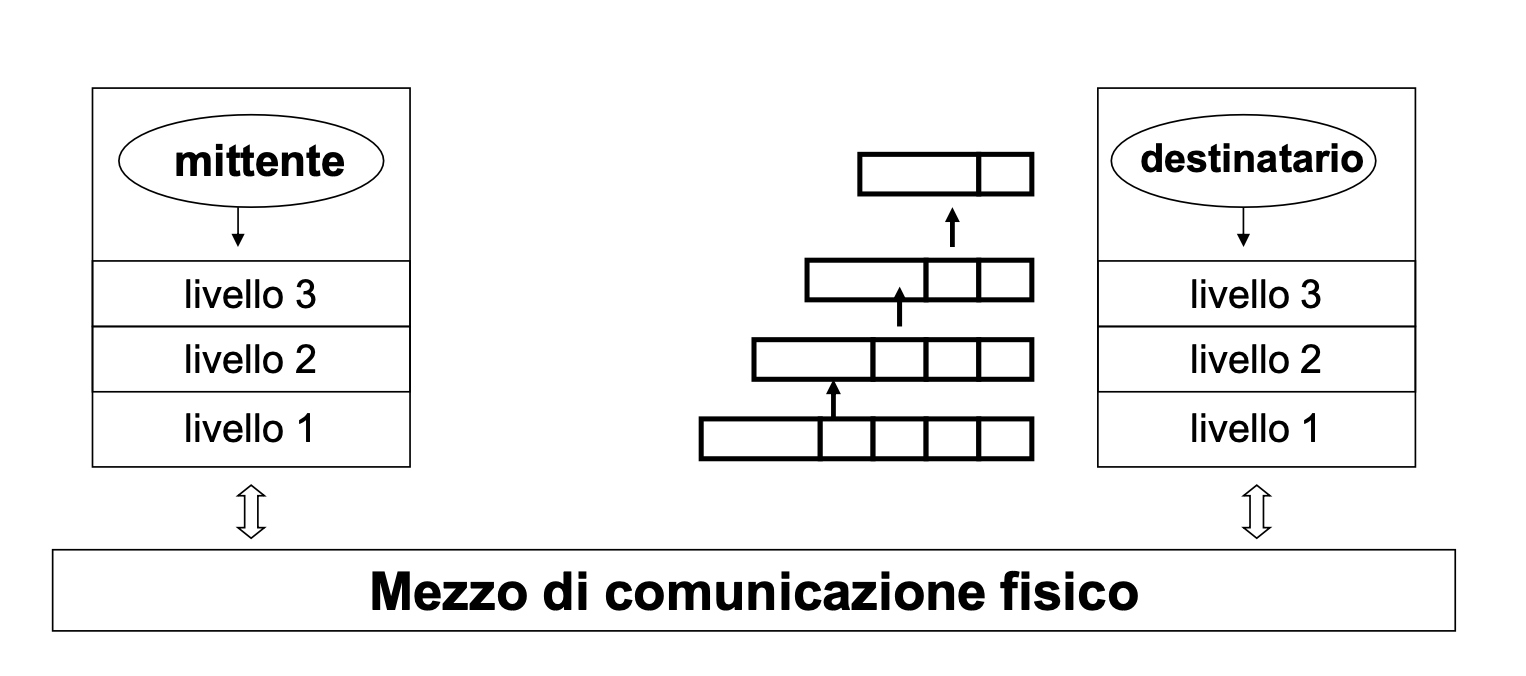
\includegraphics[width=\textwidth]{teoria_intro_13.png}
\end{minipage}

\begin{emphasize}
    \`E implicito che gli stack dei nodi host \textbf{devono essere gli stessi affinch\'e avvenga la comunicazione}
\end{emphasize}
\vspace{-5pt}
\begin{emphasize}
    Ci sono casi in cui non avviene solo questo, ma sono eccezioni oppure casi di errore (es.~un livello riceve un PDU e non riconosce il PCI)
\end{emphasize}

\begin{emphasize-blue}[frametitle={Sintesi sui protocolli}]
    \begin{enumerate}
      \item il sistema di comunicazione basato su internet richiede un \textbf{insieme di protocolli cooperanti} (stack)
      \item si identificano \textbf{relazioni gerarchiche} nelle fz. che compongono i processi di comunicazione (layering)
      \item \textbf{indipendenza funzionale} tra livelli - interfacce (e definizioni) indipendenti dall'implementazione
      \item il liv.~$n$ (sfruttando il servizio di $n-1$) fornisce un servizio a $n+1$
      \item la comunicazione avviene \textbf{logicamente tra pari}, ma in realt\`a attraversa tutti i livelli (incapsulamento)
    \end{enumerate}
\end{emphasize-blue}

Questo sistema permette la comunicazione tra processi su macchine diverse \textbf{come se fossero sulla stessa}

\subsection{Comunicazioni e standard}

Gli standard sono necessari per contesti eterogenei - da sempre in informatica si arriva a uno standard \textit{de iure} e a uno \textit{de facto}:
\begin{itemize}
  \item \textbf{ISO/OSI} (\textit{de iure}): l'organizzazione ISO (International Std.~Org.) ha definito le specifiche dello std di protocolli per l'interconnessione di nodi eterogenei (Open System Interconnection)
  \item \textbf{TCP/IP} (\textit{de facto}): nato nelle universit\`a come metodo di comunicazione estremamente efficiente, ma \textbf{non definito come standard}
\end{itemize}

\subsubsection{Stack ISO/OSI - Panoramica di funzionamento}

Lo stack ha 7 livelli:

\begin{enumerate}
  \item l.~\textbf{fisico:} gestisce i particolari meccanici ed elettrici della \textit{trasmissione fisica} di un flusso di bit
  \item l.~\textbf{di collegamento} (data link): gestisce i collegamenti tra \textit{host locali} (in LAN) (valida i dati ricevuti)
  \item l.~\textbf{di rete:} gestisce i collegamenti \textit{tra reti} $\rightarrow$ nonostante stiamo comunicando tra tante piccole reti locali, vogliamo una comunicaz.~\textit{come in una grande rete locale}
  \item l.~\textbf{di trasporto:} gestisce le com.~dei \textit{processi tra ciascun host} - \`e il protocollo con cui si interfacciano le applicazioni
  \begin{emphasize}
      I livelli superiori presentano funzionalit\`a di aiuto alle applicazioni
  \end{emphasize}
  \item l.~\textbf{di sessione:} consente a utenti su macchine eterogenee di stabilire sessioni, mantenendo lo stato (es.~A vuole comunicare con B - come tratto i msg? sono tutti per la stessa app/tutti eterogenei? $\rightarrow$ B deve implementare uno stato) (sessione \`e il termine tecnico per definire questo comportamento)
  \item l.~\textbf{di presentazione:} manipola le informazioni per presentarle nel modo migliore possibile su ciascun dispositivo (es.~conversioni di codifica)
  \item l.~\textbf{di applicazione:} livello concettuale, in cui semplicemente inseriamo l'applicazione (fornisce un'interfaccia std per i programmi applicativi)
\end{enumerate}

\begin{center}
  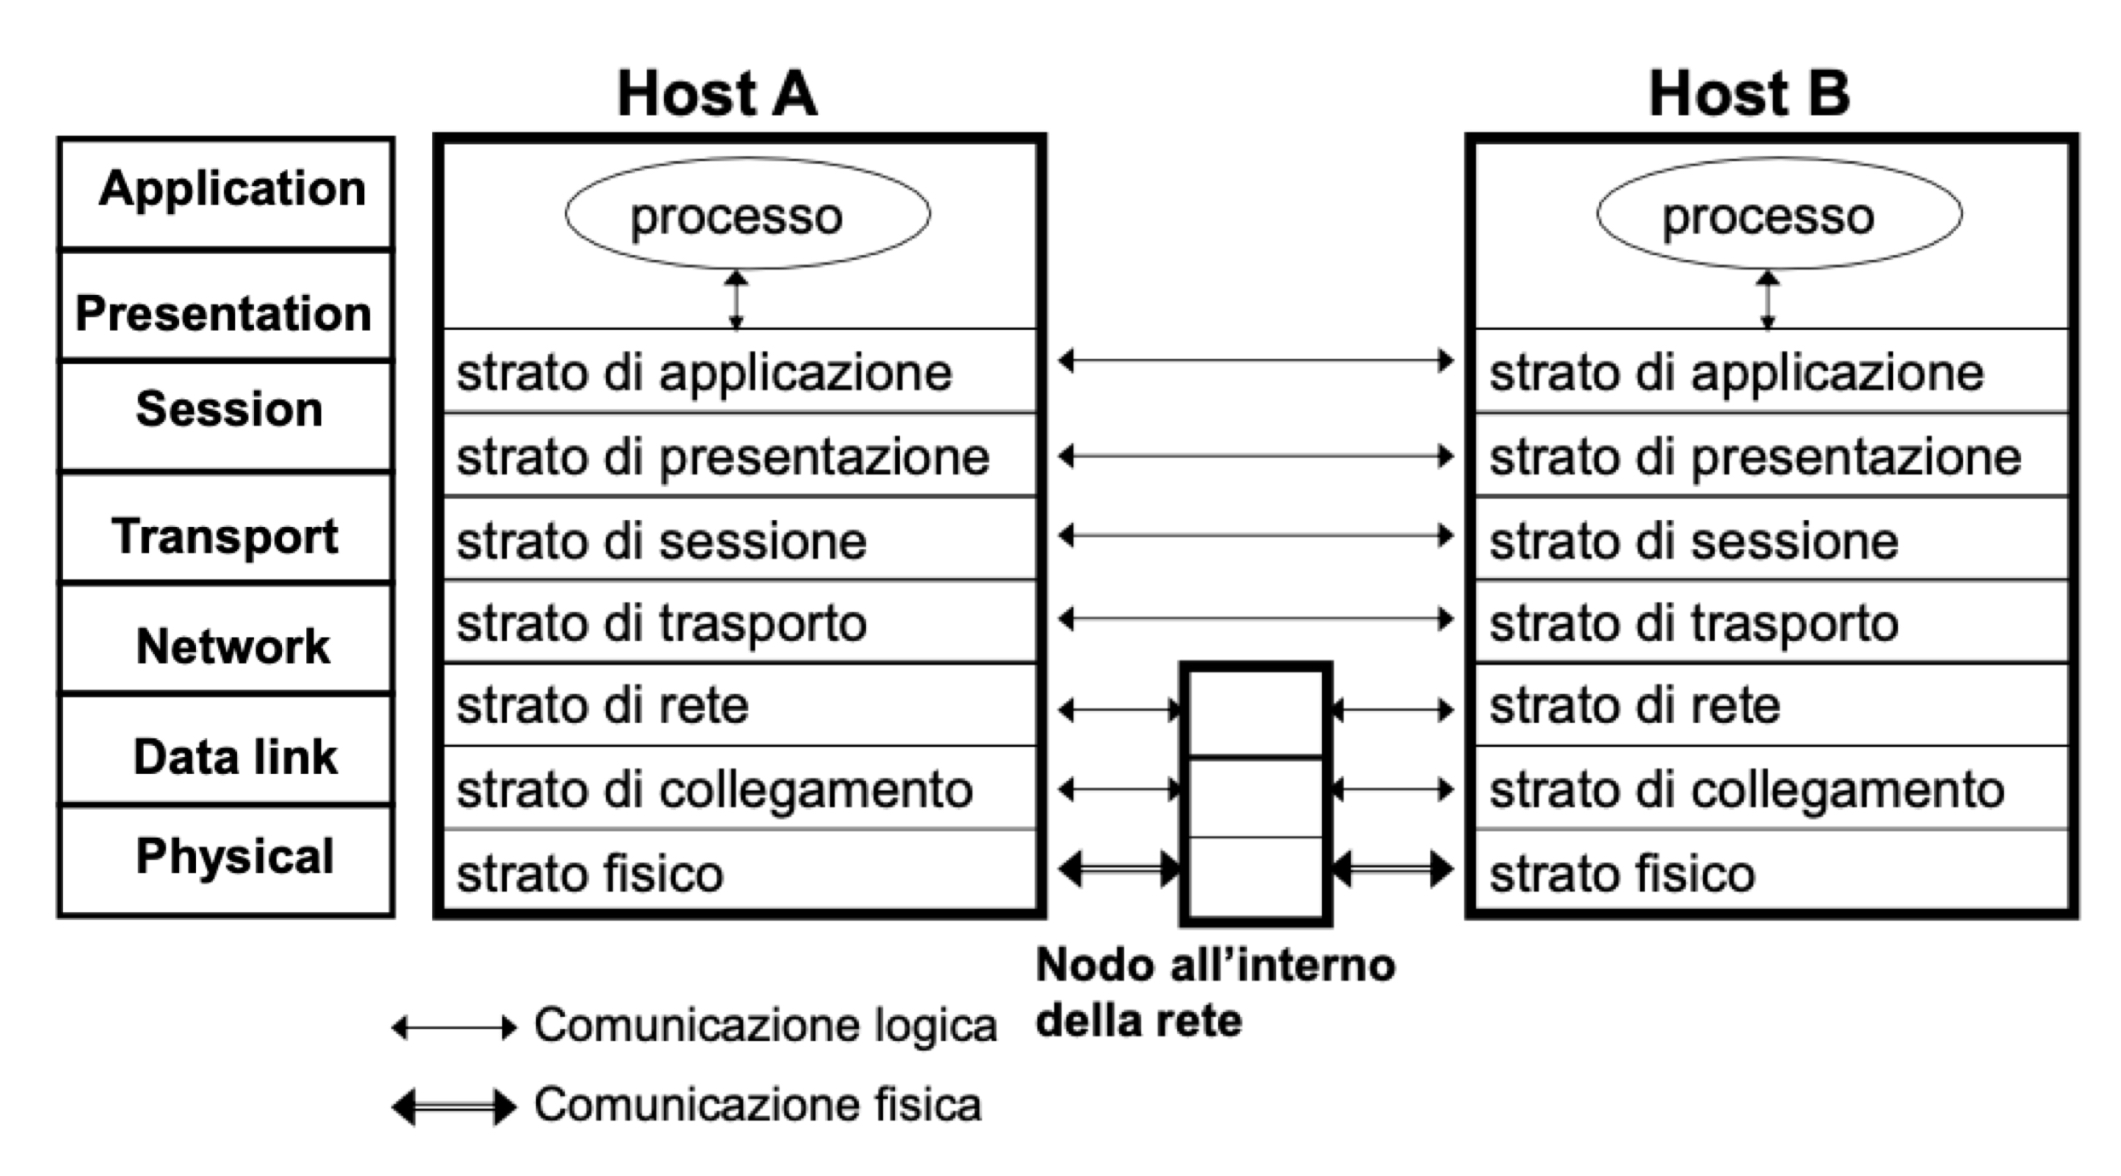
\includegraphics[width=.5\textwidth]{teoria_intro_14.png}
  \captionof{figure}{Schema dello stack ISO/OSI}
\end{center}

\begin{emphasize-blue}[frametitle={Reminder}]
    Per ciascuna comunicazione, sono aggiunti/tolti i PCI di ogni livello $\rightarrow$ 7 livelli sono \textbf{troppi} - anche per questo si afferma TCP/IP (ne ha 5)
\end{emphasize-blue}

\begin{multicols}{2}
Il motivo principale per cui ha prevalso TCP/IP \`e che \`e uno stack \textbf{open, senza controllo centralizzato, e in generale pi\`u semplice e meno costoso}. Inoltre, aveva gi\`a un'API \textbf{funzionante}
\begin{emphasize}
    Nonostante studieremo lo stack TCP/IP, per convenzione usiamo i numeri dei liv.~ISO/OSI\\
    es.~per dire che lavoriamo a liv.~rete usiamo \textbf{3 e non 2}
\end{emphasize}
\centering
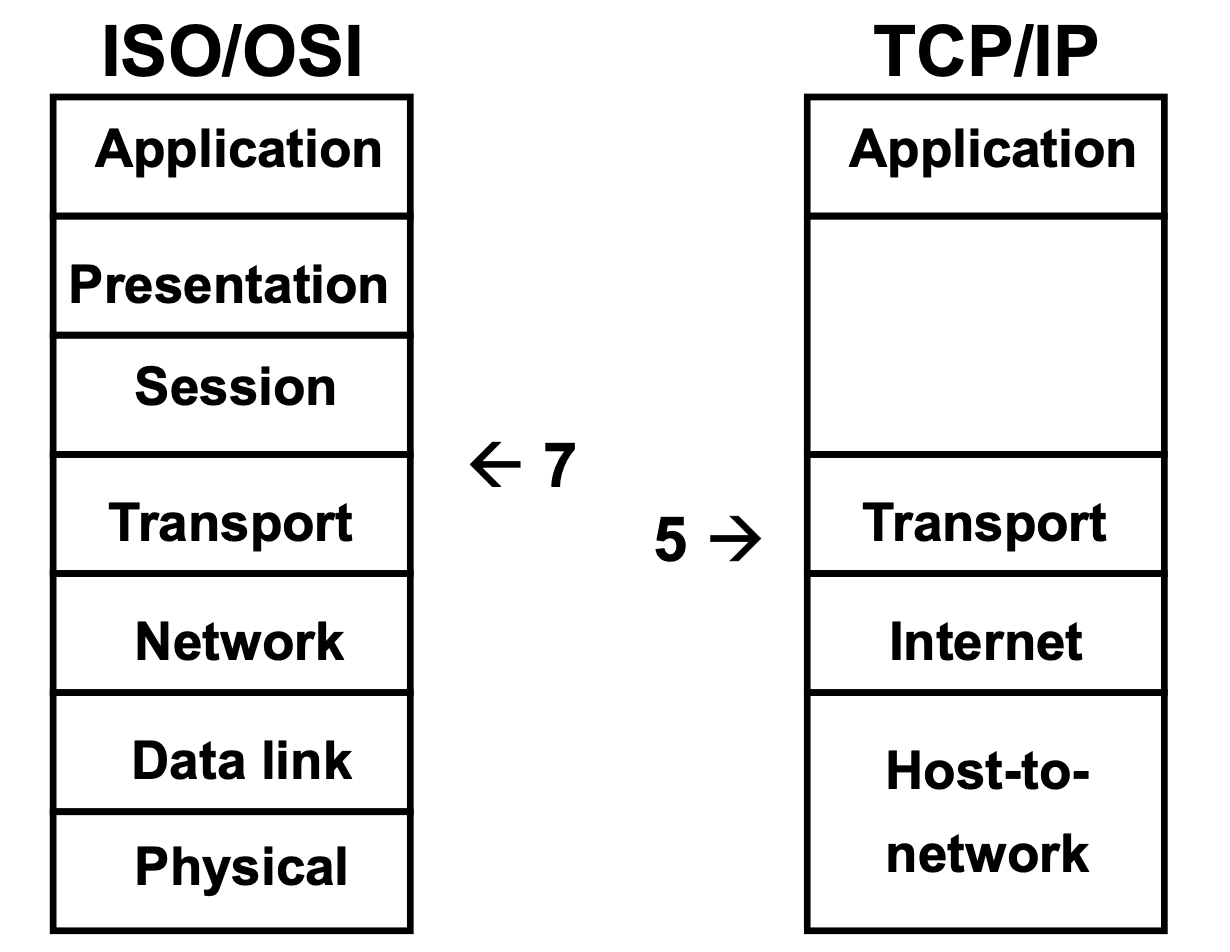
\includegraphics[width=.9\linewidth]{teoria_intro_15.png}
  \captionof{figure}{Confronto tra ISO/OSI e TCP/IP}
\end{multicols}

\subsubsection{Stack TCP/IP}

\paragraph{Definizione dei livelli}~\\
\noindent\begin{minipage}[c]{.5\textwidth}
\begin{itemize}
  \item[4.] \textbf{trasporto}: supporta i trasferimenti fra processi in esecuzione su host
  \item[3.] \textbf{rete}: trasferisce i pacchetti dal nodo mittente al destinatario
  \item[2.] \textbf{link}: effettua i trasferimenti dei dati tra componenti della rete confinanti
  \item[1.] \textbf{fisico}: trasferisce bit "sul cavo"
\end{itemize}
\end{minipage}
\begin{minipage}[c]{.5\textwidth}
  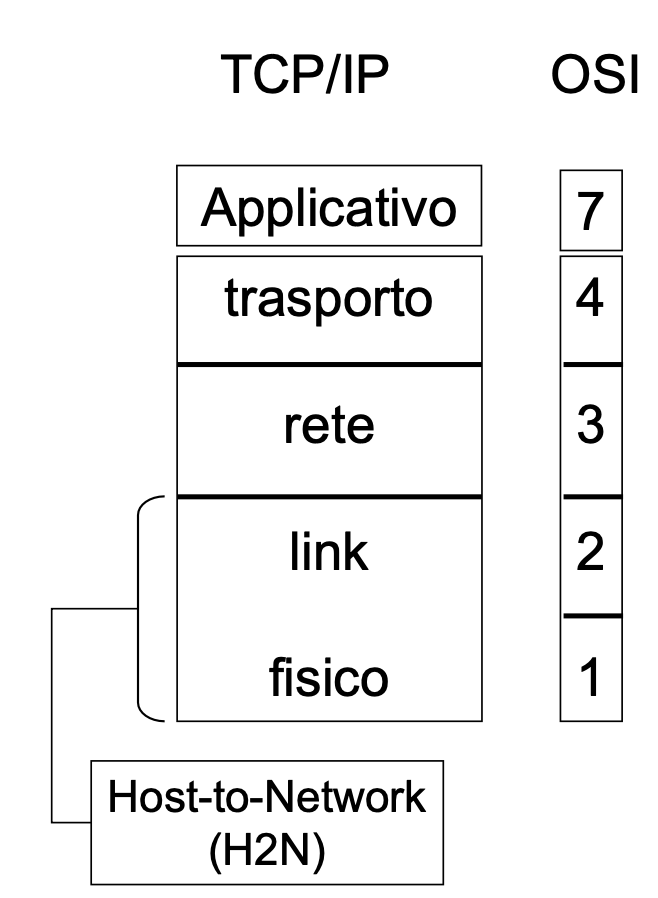
\includegraphics[width=.35\textwidth]{teoria_intro_16.png}
  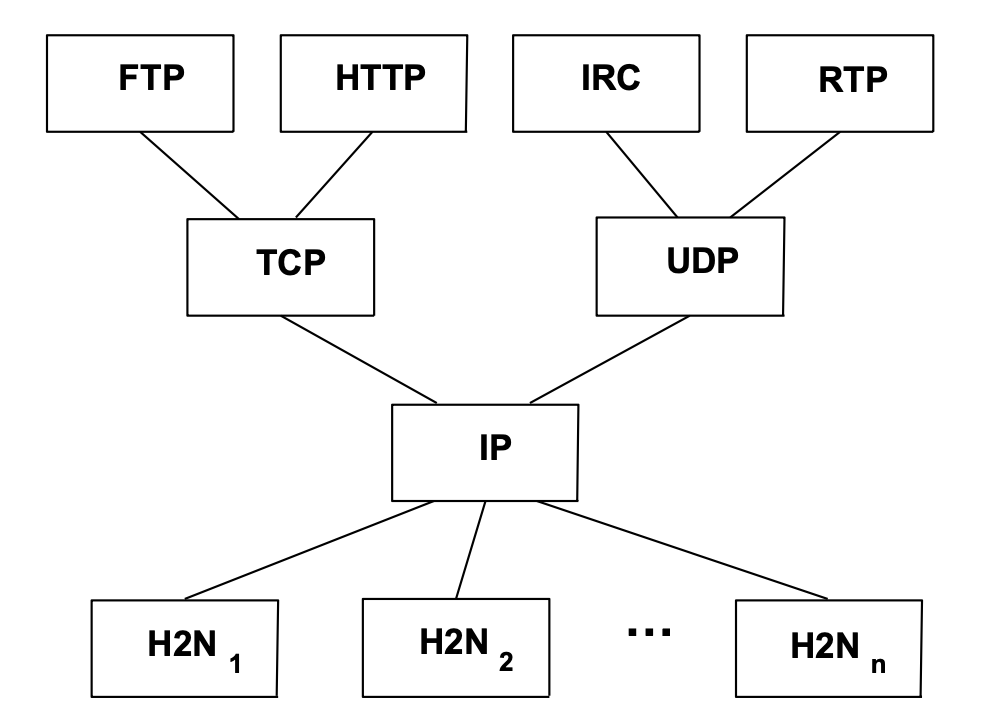
\includegraphics[width=.65\textwidth]{teoria_intro_17.png}
  \captionof{figure}{Schema dello stack e implementazioni}
\end{minipage}\\

I pr.~del livello H2N comunicano con il pr.~del livello network, cio\`e IP

\begin{multicols}{2}
A liv.~trasporto:
\begin{itemize}
  \item TCP - per creare comunicazioni \textbf{affidabili}
  \item UDP - non d\`a affidabilit\`a
\end{itemize}

A liv.~applicativo:
\begin{itemize}
  \item HTTP - rete
  \item RTP - comunicazioni real-time
\end{itemize}
\end{multicols}

\begin{emphasize}
    C'\`e molto altro, che vedremo in seguito o proprio non vedremo
  \end{emphasize}
  \vspace{-10pt}
\begin{emphasize-blue}
    Ricordiamoci che l'obiettivo \`e sempre far comunicare 2 host, e che i nodi intermedi analizzano il pacchetto a profondit\`a differenti
\end{emphasize-blue}

Quando dobbiamo definire i vari nodi, li definiamo in base a ci\`o che implementano:
\begin{itemize}
  \item \textbf{host}: implementa tutto lo stack
  \item \textbf{switch e bridge}: nodi di l.~2 (implementano fino a 2)
  \item \textbf{router}: liv.~3
  \item in generale, disp.~di livello $n$ implementano lo stack fino al liv.~$n$, ma possono esserci eccezioni (es.~switch di liv.~3)
\end{itemize}

\noindent\begin{minipage}[t]{.5\textwidth}
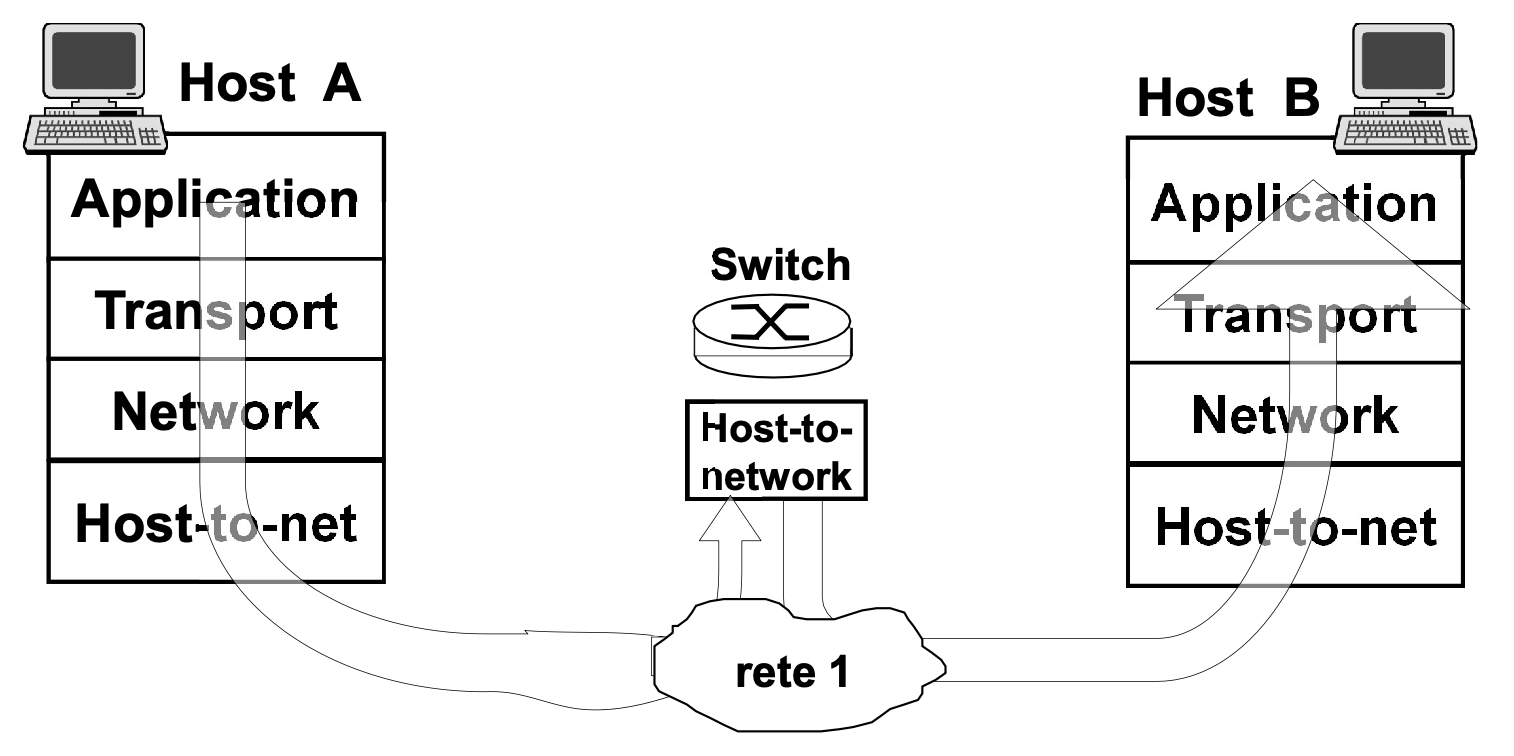
\includegraphics[width=\textwidth]{teoria_intro_18.png}
\captionof{figure}{Comunicazione a liv.~2 (LAN)}
\end{minipage}
\begin{minipage}[t]{.5\textwidth}
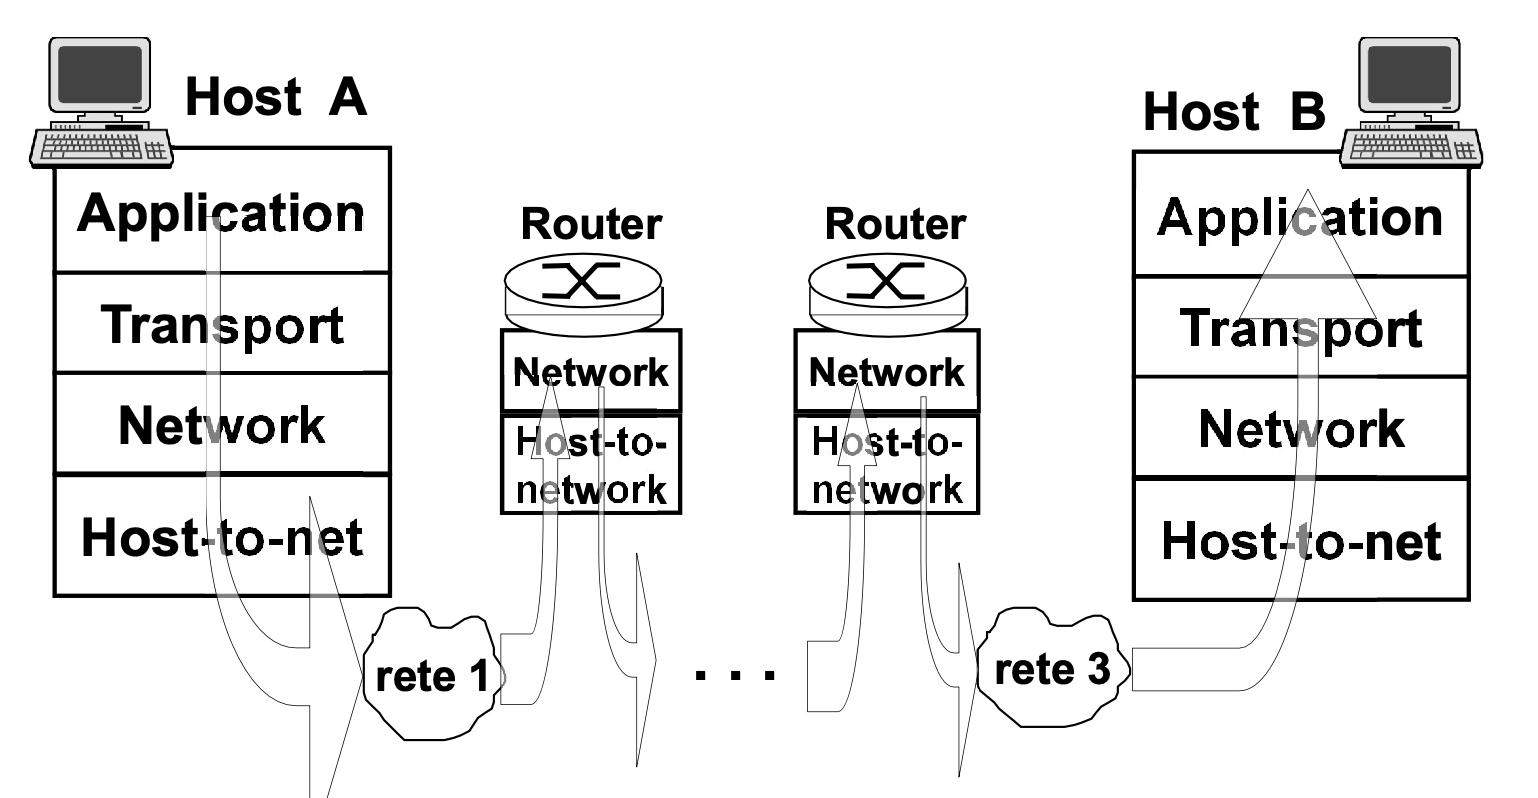
\includegraphics[width=\textwidth]{teoria_intro_19.png}
\captionof{figure}{Comunicazione a liv.~3 (Internet)}
\end{minipage}

\begin{emphasize}
    Il motivo per cui si usano disp.~di livello pi\`u basso \`e \textbf{il costo a parit\`a di velocit\`a di gestione del traffico}
\end{emphasize}

\subsubsection{Problemi di instradamento e condivisione delle risorse}

\begin{itemize}
  \item i problemi di instradamento si risolvono tramite lo \textbf{stack}
  \item per la condivisione delle risorse usiamo il \textbf{multiplexing}
  \begin{itemize}
    \item[$\rightarrow$] ogni volta che pi\`u dispositivi vogliono \textbf{comunicare tramite un canale condiviso}
    \item la realizzazione dipende dal \textbf{paradigma} di com.~e dalle \textbf{caratteristiche del canale} di com.
  \end{itemize}
\end{itemize}

\subsubsection{Modalit\`a di trasferimento dati}

\paragraph{Circuit switching}~\\

Alla base di protocolli analogici: 1 circuito virtuale $\forall$ comunicazione
\begin{itemize}
  \item poco adatto a Internet: prevede l'\textbf{assegnazione statica del percorso}
  \item[$\rightarrow$] poco efficiente in contesti dinamici
  \item Time o Frequency Division Multiplexing sono due esempi, entrambe dividono la risorsa a disposizione ma non permettono modifiche al percorso
\end{itemize}

\paragraph{Packet switching}~\\

Alla base di internet: dati suddivisi in \textbf{pacchetti} ed inviati in rete
\begin{itemize}
  \item un pacchetto usa \textbf{tutta la capacit\`a trasmissiva} di un link
  \item l'accesso al mezzo \textbf{non \`e temporizzato} ($\neq$TDM) e \textbf{non \`e a prenotazione} $\rightarrow$ le risorse sono usate in base alla necessit\`a
  \item[$\rightarrow$] accessi \textbf{non decisi a priori}: paradigma la cui efficacia \`e stata dim.~ dalla teoria delle reti di code (Kleinrock, 1961)
  \item segue un principio di \textit{MUX-ing statistico a suddivisione di tempo}: pacchetti da sorgenti diverse sono "mescolati" sullo stesso link senza slot temporali dedicati e occupando tutta la banda disponibile
\end{itemize}

Non essendoci garanzia di disponibilit\`a della risorsa, possiamo incontrare 2 problemi principali:\\

\noindent\begin{minipage}[c]{.6\textwidth}
\begin{itemize}
  \item \textbf{collisione}: host $\neq$ vogliono comunicare nello \textbf{stesso esatto momento}
    \begin{itemize}
      \item[$\rightarrow$] fenomeno a livello locale
  \end{itemize}
  \item \textbf{congestione}: molti pacchetti arrivano \textbf{contemporaneamente ad un nodo intermedio}
    \begin{itemize}
      \item[$\rightarrow$] malfunz.~a livello non locale (buffer dei router)
      \item es.~dopo una com.~corretta a livello locale, i pacchetti arriveranno ad un router che li \textit{smister\`a} in base alla destinazione; per farlo li \textit{analizza} e li mette su dei \textit{buffer di uscita} $\rightarrow$ congestione \textbf{quando i buffer sono pieni} ed \`e \textbf{obbligato a scartare un pacchetto}
    \end{itemize}
\end{itemize}
\end{minipage}\hfill
\begin{minipage}[c]{.35\textwidth}
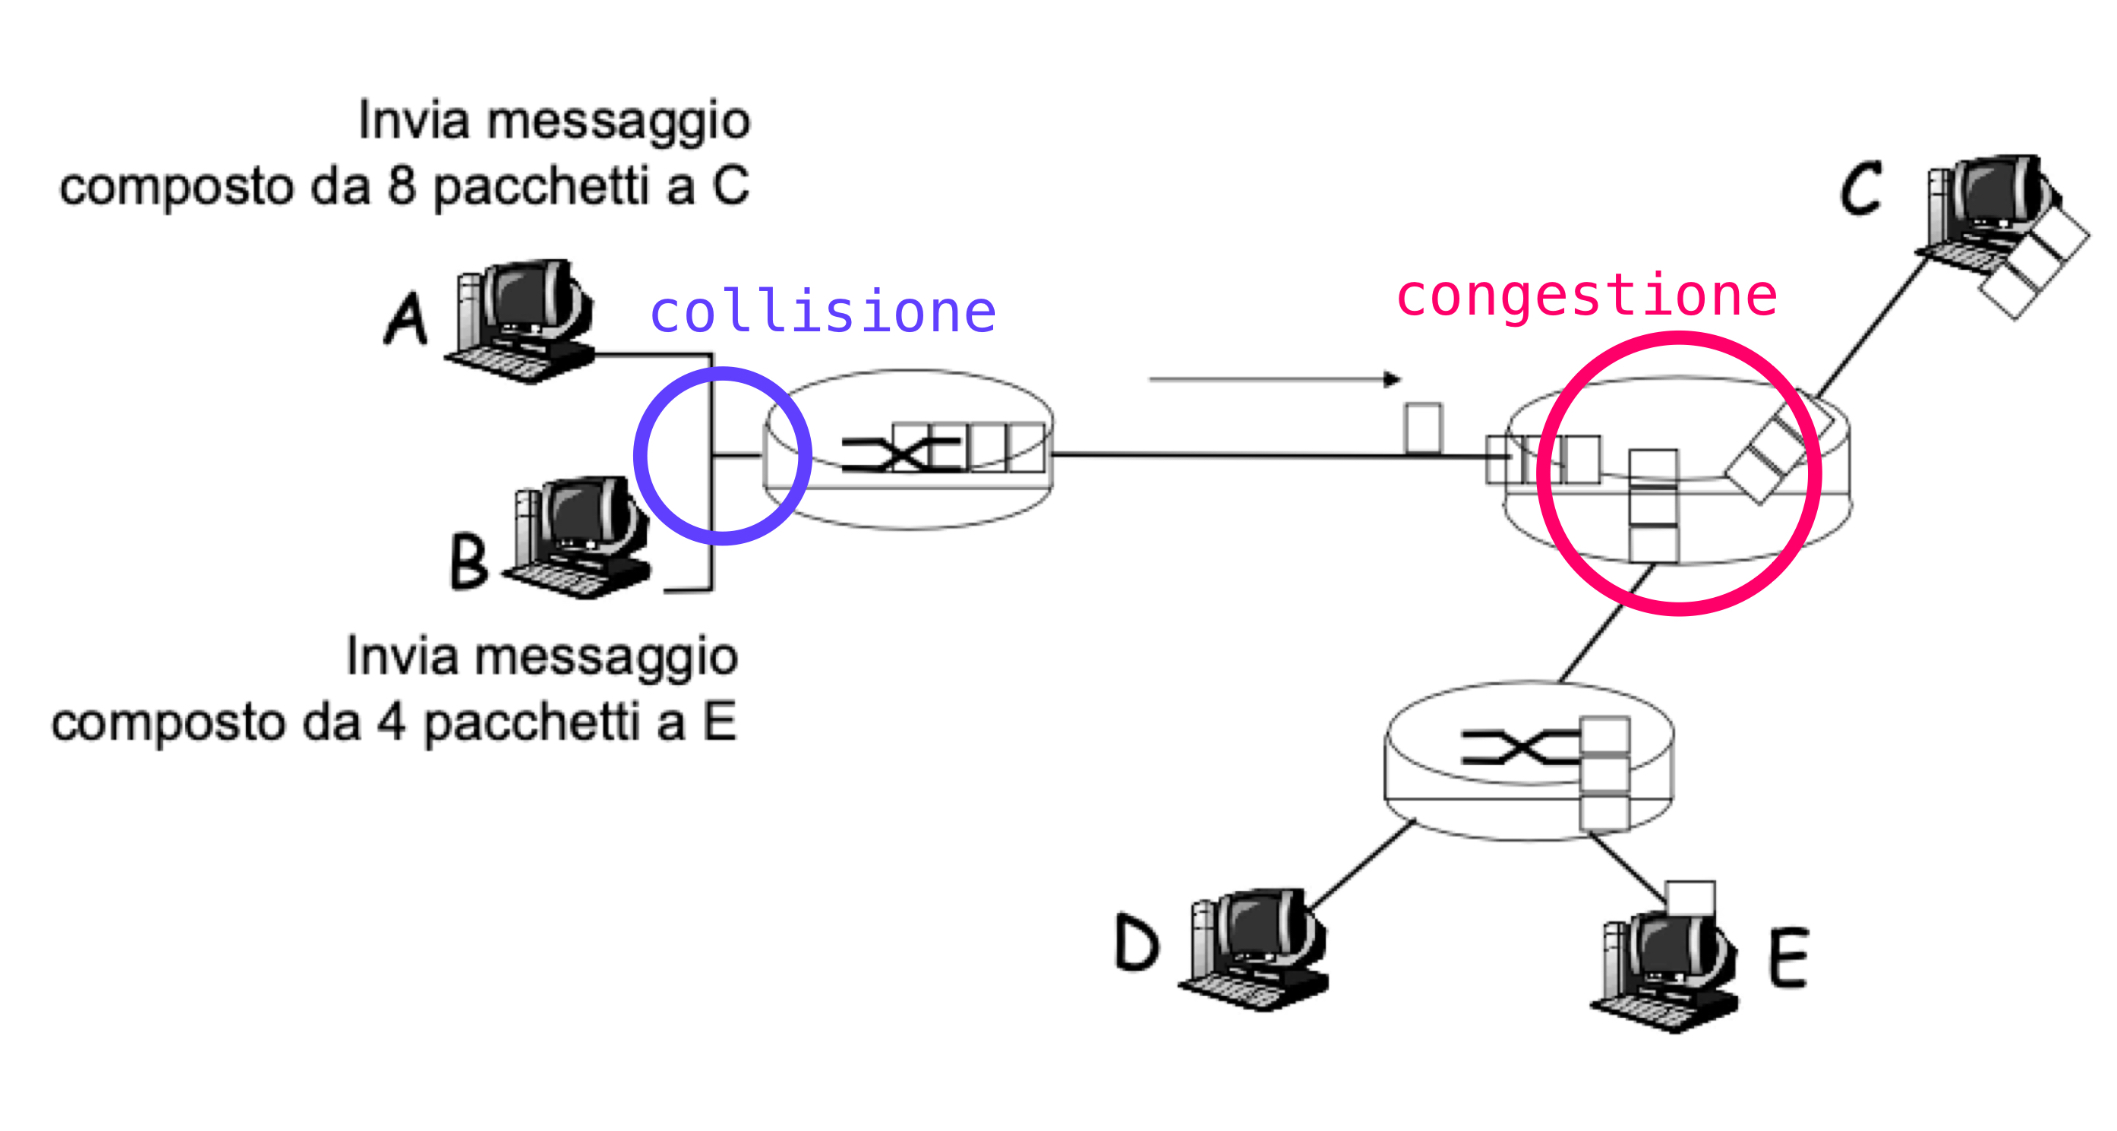
\includegraphics[width=\textwidth]{teoria_intro_20.png}
\captionof{figure}{Dove avvengono i malfunzionamenti locali (\textit{collisione}) e non (\textit{congestione})}
\end{minipage}

\subsubsection{Metrica di prestazione}

\begin{itemize}
  \item principalmente usiamo la \textbf{larghezza di banda} (o bandwidth o banda di trasmissione), tipicamente in multipli di bit/secondo (es. Kbps o Kbit/s, Mbps, Gbps, ...)
  \item[$\rightarrow$] identifica la velocit\`a \textbf{a liv.~fisico} (a liv.~applicativo risulter\`a inferiore)
  \item la massima velocit\`a ottenibile \`e detta \textbf{v.~nominale} $\rightarrow$ non la raggiungo es.~quando uso un canale di comunicazione condivisa
  \item[es.] link a 1 Mbps (nominale), ciascun utente richiede 0.1 Mbps quando trasmette ed \`e attivo il 10\% del tempo
  \begin{itemize}
    \item circuit sw.: \textbf{max 10 utenti}
    \item packet sw.: con \textbf{35 utenti}, la prob.~che \textit{10+ trasmettano contemporaneamente} \`e \textbf{~0.04\%} $\rightarrow$ \textbf{rischio minimo}
  \end{itemize}
\end{itemize}

\newpage % FINE CAPITOLO

\section{Livello H2N (Host-2-Network)}

\noindent\begin{minipage}[c]{.55\textwidth}
Unione dei livelli 1 e 2 dello stack ISO/OSI

Affronta le problematiche di
\begin{itemize}
  \item \textbf{interconnessione} tra 2+ host
  \item \textbf{trasmissione dati} tra host connessi direttamente
  \item \textbf{conessione a Internet} di un host
\end{itemize}
Nello stack TCP/IP (non in ISO/OSI) la \textbf{modalit\`a} di interconnessione, la relativa \textbf{tecnologia} ed i \textbf{protocolli} per la trasmissione di dati tra host interconnessi sono \textbf{strettamente dipendenti}
\end{minipage}\hfill
\begin{minipage}[c]{.4\textwidth}
  \begin{tabular}{| p{.5\textwidth} | p{.5\textwidth} |}
    \hline
    \cellcolor{gray!20} Modalit\`a & \cellcolor{gray!20} Tecnologie/Protocolli \\
    \hline
    \hline
    LAN wired & Ethernet, token ring, ... \\
    LAN wireless & 802.11x \\
    PAN & Bluetooth, ... \\
    mediante modem & SLIP, ... \\
    WAN wireless & GSM, LTE, ... \\
    \hline
  \end{tabular}
  \captionof{table}{Esempi concreti di tecnologie e protocolli usati nelle varie modalit\`a}
\end{minipage}

\begin{emphasize}[frametitle={Premessa}]
    I servizi offerti da protocolli H2N $\neq$ possono essere \textbf{diversi}! Ad es., possono \textbf{garantire} o \textbf{no} l'\textbf{affidabilit\`a} della consegna di un pacchetto (pur facendo parte dello stesso livello dello stack)\\
    $\rightarrow$ il liv.~network deve essere in grado di garantire l'arrivo dei pacchetti \textbf{anche in presenza di pr.~H2N $\neq$}
\end{emphasize}
\begin{emphasize-blue}[frametitle={Osservazione}]
   Solitamente i collegamenti \textbf{wired} sono \textbf{pi\`u affidabili} rispetto a quelli \textbf{wireless}
   \begin{itemize}
     \item c.~\textbf{wireless}: pi\`u soggetti a malfunzionamenti $\implies$ protocolli \textbf{pi\`u sicuri e complessi}
     \item c.~\textbf{wired}: pi\`u sicuri fisicamente $\implies$ protocolli \textbf{meno sicuri e pi\`u semplici}
   \end{itemize}
   Studieremo il pr.~Ethernet, che essendo pensato per reti cablate (sicure fisicam.) \`e generalmente \textbf{inaffidabile}
\end{emphasize-blue}

Alcune definizioni:

\paragraph{Modalit\`a di trasmissione}~\\

Dipendono da chi sono i nodi terminali che vogliono comunicare
\begin{itemize}
  \item \textbf{unicast}: 1 a 1 (mittente-destinatario)
  \item \textbf{multicast}: 1 a molti (vogliamo comunicare con \textbf{tutti i destinatari})
  \item \textbf{anycast}: 1 a "almeno 1" (sufficiente 1 solo ricevente)
  \item \textbf{broadcast}: 1 a tutti gli altri nodi (multicast dove molti = tutti)
\end{itemize}


\end{document}
